\graphicspath{{background/fig/}}

\chapter{Background}
\label{chap:background}

% ***************************************************
% SECTION 1
% ***************************************************
\section{The Automatic Speech Recognition Task}\label{sec:background}
Automatic speech recognition (ASR), also known as speech recognition, 
involves predicting the sentence for a given speech recording.
For example, given a recording of a person saying the sentence ``The quick brown fox jumps over the lazy dog.'',
the goal of ASR is to predict each character in the sentence and to make as few mistakes as possible.

The general approach for ASR involves two steps.
In the first step, we convert speech recordings into a higher-dimensional feature representation called \emph{speech features}.
Then, in the second step we use supervised learning techniques to map speech features 
to a sequence of characters that are merged into a sentence.

Computing speech features is useful because recording data is difficult to interpret. 
Recording data, or audio data, consists of a one-dimensional array of integers called \emph{samples}.
The sequence of samples represent amplitude measurements of the recorded sound wave. 
Note that sound is a continuous wave function, but a recording is a discretized version of the original sound that was recorded.
This is explained by Figure \ref{fig:wave} below, which is an oversimplification of what an audio file represents.

\begin{figure}[h!]
    \centering
    \captionsetup{justification=centering}
    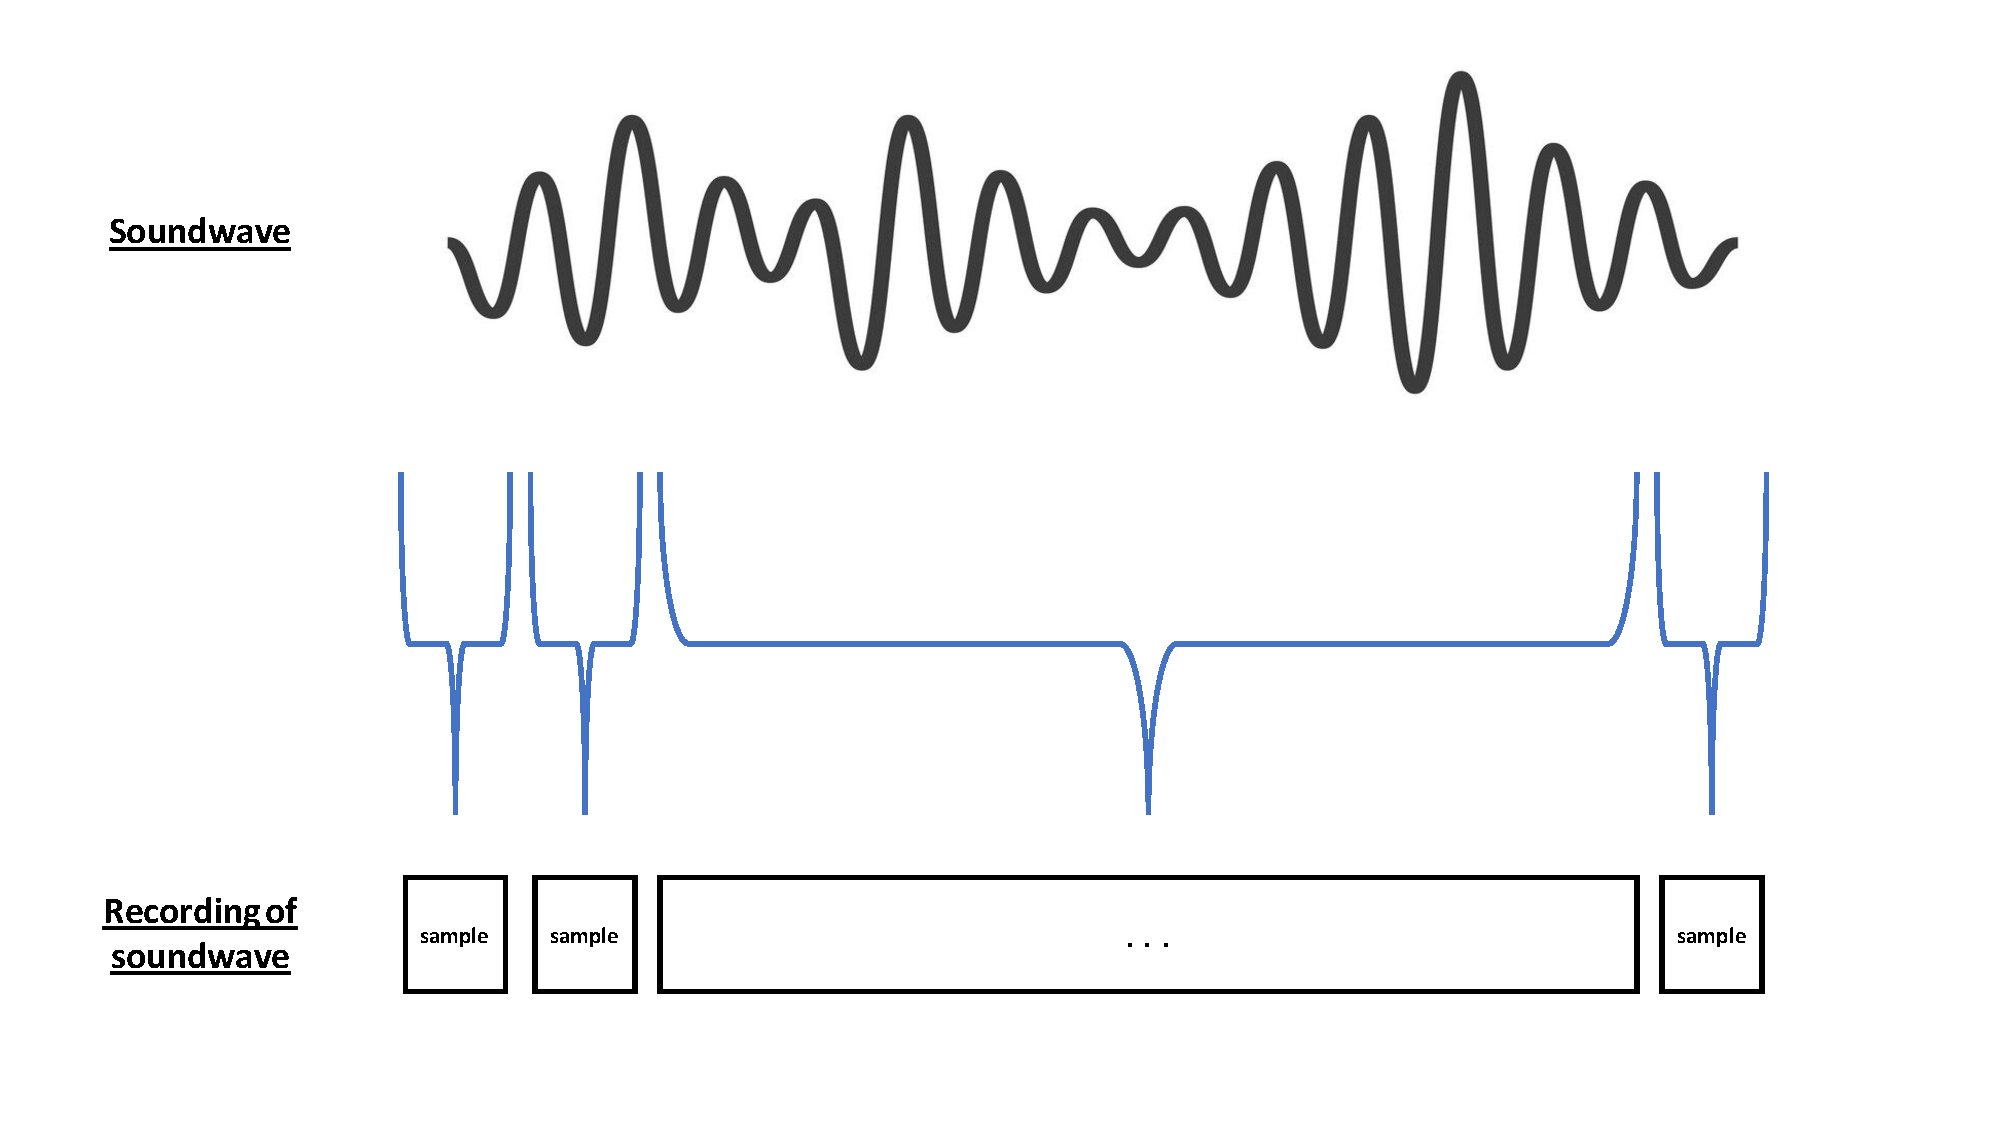
\includegraphics[width=0.76\textwidth]{wave.pdf}
    \caption{A diagram that explains what the data of a recording, or audio data, represents.}
    \label{fig:wave}
\end{figure}

The issue is that mapping a sequence of samples to a sequence of characters is difficult. 
Therefore, it is common in ASR and other speech-related tasks to first convert audio data into speech features.
A common technique used to compute speech features is to transform the audio data from the amplitude-time domain 
to the frequency-time domain using the Fast Fourier Transform (FFT) algorithm \cite{cochran1967fast}, \cite{cooley1969fast}.

In this study, we will discuss an approach to obtain speech features using self-supervised learning.
Before discussing this approach, we would like to discuss the significance of choosing the speech audio data 
used to train and evaluate ASR models.

\subsection{Speech recognition data}
The first step of creating an ASR model is to prepare a training, validation, and test dataset. 
A single dataset entry consists of a speech recording (of a spoken sentence) and the corresponding text of the spoken sentence.
The following paragraphs demonstrate why the choice of training and validation data 
has a significant effect on the accuracy and generalization ability of ASR models.

\paragraph*{The amount of training data.} The more data that is available during training the better the ability
of the ASR model to generalize. A small dataset (with few unique voices) may lead to overfitting to the specific 
voices in the dataset.

\paragraph*{The difference between read and conversational speech.} 
We believe that humans tend to speak more clearly when reading text from a transcript, in comparison to conversational speech.
Recent ASR models obtain very low error rates for recordings of read speech \cite{jurafskyspeech}.
However, ASR for recordings of conversational speech is still a major challenge \cite{jurafskyspeech}.

\paragraph*{Differences in accents.} 
The accent of the speaker, which depends on the gender, age, and ethnicity of the speaker may also influence the generalization ability of ASR models. 
Generally, male voices have a lower pitch than female voices, and adults have a lower pitch than children.

\paragraph*{The audio quality of speech recordings.} 
The position of the microphone, 
the quality of the microphone, 
the number of microphones available, 
and the presence of background noise contribute towards the audio quality of speech recordings.
\\
\\
In the following section, we discuss the speech feature extraction technique used in this study.

% ***************************************************
% SECTION 2
% ***************************************************
\newpage
\section{wav2vec 2.0}
wav2vec 2.0 provides a framework for learning speech representations using unlabeled speech data.
wav2vec 2.0 can be applied to a variety of speech-related tasks such as speech recognition, speech translation,
and speech classification.
It proves to be particularly useful in cases where a lot of unlabeled data is available, but not much labeled data is available.
The authors show that using just ten minutes of labeled data and pre-training
on 53K hours of unlabeled data still achieves $4.8$/$8.2$ WER on the clean/other test sets of Librispeech~\cite{panayotov2015librispeech}.

The general two-step approach for using wav2vec 2.0 for any speech-related task is the following.
First train (or ``pre-train'') the wav2vec 2.0 model using unlabeled data, which
will give you a model that converts audio data into speech features.
In the second step the model is fine-tuned on a downstream task using labeled data. 
Fine-tuning wav2vec 2.0 (\ref{subsec:finetune}) for speech recognition involves replacing the head of the 
pre-trained model with an appropriate loss function such as CTC (\ref{sec:ctc}).

\begin{figure}[h!]
    \centering
    \captionsetup{justification=centering}
    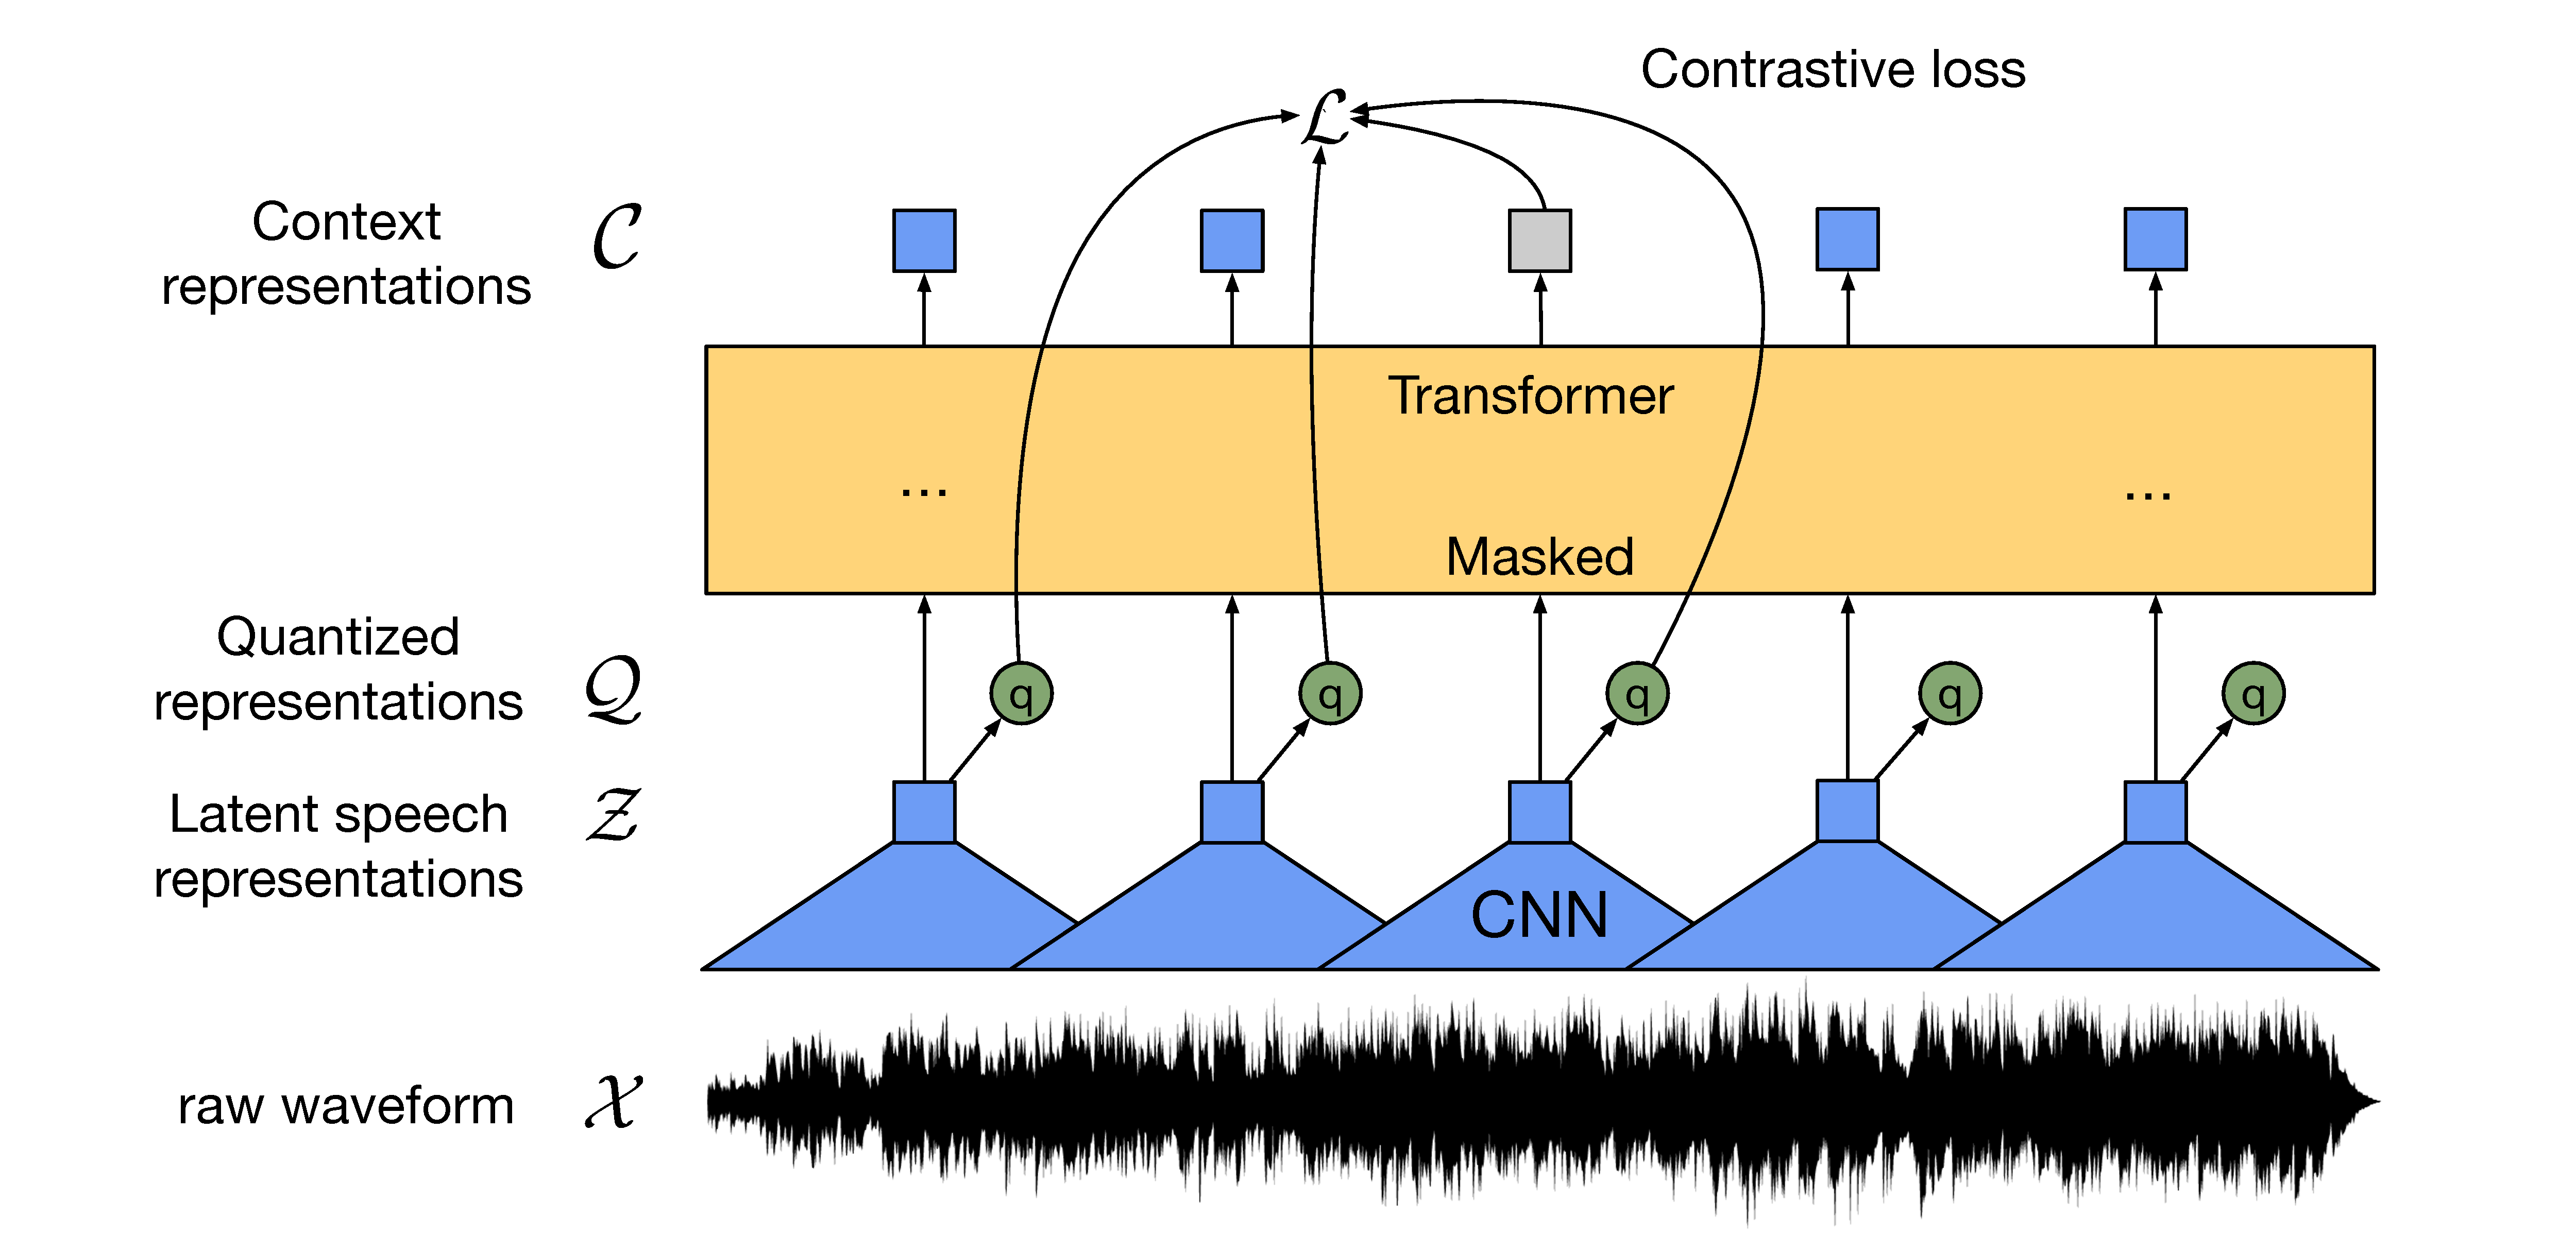
\includegraphics[width=\textwidth]{wav2vec2architecture.pdf}
    \caption{A visualization of the network architecture of wav2vec 2.0 \cite{baevski2020wav2vec}. \hl{TODO}: create own version of this.}
    \label{fig:wav2vec2_architecture}
\end{figure}

The wav2vec 2.0 architecture is described by the network diagram in Figure~\ref{fig:wav2vec2_architecture}.
There are three important components of the wav2vec 2.0 architecture:
the feature encoder, the quantization module, and the context network.
The objective of wav2vec 2.0 becomes clear only after understanding each of the three
components. Therefore, we explain how to pre-train wav2vec 2.0 only after explaining
the three components in detail.

\newpage
\subsection{Feature encoder}
The feature encoder maps raw audio data to latent speech representations: $f: \mathcal{X} \rightarrow \mathcal{Z}$.
Thus, the feature encoder $f$ maps a sequence of audio samples $\mathbf{x}^{(1)}, \dots \mathbf{x}^{(N)}$ into a sequence of latent feature vectors $\mathbf{z}^{(1)}, \dots, \mathbf{z}^{(t)}$.


The audio data is scaled to have zero mean and unit variance before going into the feature encoder. 
The feature encoder consists of seven convolutional blocks, where each convolutional block contains a temporal\footnote{One-dimensional convolutional layer designed for sequential data.} convolutional layer, 
a layer normalization layer, and the GELU activation function.

Each temporal convolutional layer contains 512 channels. 
The strides of the seven temporal convolutional layers are $(5,2,2,2,2,2,2)$ and the kernel widths are $(10,3,3,3,3,2,2)$.
The strides used results in each $\mathbf{z}^{(t)}$ representing $25$ms of audio (or $400$ input samples),
strided by about $20$ms.

Layer normalization scales the logits after each convolutional layer to have zero mean and unit variance, which has shown to increase the chances of earlier convergence.
GELU has become a popular activation function for NLP related tasks



\subsection{Quantization module}
The quantization module maps the latent speech features into discrete speech units: $h: \mathcal{Z} \rightarrow \mathcal{Q}$.
Speech is sound, and sound is represented as a continuous function. We would like to use Transformers and so continuous representations will not work. 
Unlike written language, which can be discretized into tokens such as characters or sub-words, speech does not have natural sub-units \cite{bgn2021illustrated}. 
The quantization module is a method in which discrete speech units are automatically learned using product quantization.

To perform product quantization, the quantization module uses $G$ \emph{codebooks}, where each codebook contains $V$ \emph{codebook entries} $\mathbf{e}_{1}, \dots, \mathbf{e}_{V}$.

The following steps describe the process of automatically assigning a discrete speech unit to each latent speech feature $\mathbf{z}^{(t)}$:
\begin{enumerate}
    \item Transform $\mathbf{z}^{(t)}$ into $\mathbf{l}^{(t)} \in \mathbb{R}^{G \times V}$ using a linear transformation.
    \item Choose one codebook entry $\mathbf{e}_g$ for each codebook $g = 1, \dots, G$, based on the values of $\mathbf{l}^{(t)}$.
    \item Concatenate the codebook entries $\mathbf{e}_1, \dots, \mathbf{e}_G$.
    \item Transform the resulting vector into $\mathbf{q}^{(t)} \in \mathbb{R}^{f}$ using another linear transformation.
\end{enumerate}
The two linear transformations are feed-forward neural networks $\text{FF}_1: \mathbb{R}^{f} \rightarrow \mathbb{R}^{G \times V}$ and $\text{FF}_2: \mathbb{R}^{d} \rightarrow \mathbb{R}^{f}$.
In the second step above, the codebook entry $\mathbf{e}_g$ is chosen as the one with the argmax of the logits $\mathbf{l}$. Choosing the codebook entries in this way is non-differentiable.
Fortunately, we can use the Gumbel softmax to choose codebook entries in a fully differentiable way. 
$\mathbf{e}_g$ is chosen as the entry that maximizes
\begin{equation}
    p_{g, v} = \dfrac{\exp{\left(\mathbf{l}^{(t)}_{g, v} + n_v\right)}/\tau}{\sum\limits_{k=1}^{V} \exp{\left(\mathbf{l}^{(t)}_{g, k} + n_k\right)}/\tau},
\end{equation}
where $\tau$ is a non-negative temperature, $n = -\log{(-\log{(u)})}$, and $u$ are uniform samples from $\mathcal{U}(0, 1)$.
During the forward pass, codeword $i$ is chosen by $i = \text{argmax}_j p_{g,j}$ and in the backward pass, the true gradient of the Gumbel softmax outputs is used.



\subsection{Context network}
% Explain what it is and its purpose
The context network creates contextualized representations from the feature encoder outputs.
The main component of the context network is a Transformer encoder \cite{transformer}.
Due to the popularity of Transformers we have ommited a detailed explanation of the Transformer architecture. 
Interested readers should refer to \cite{transformer} as well as guides such as \cite{alammar2018illustrated}.

% Explain architecture further
The following steps describe how the latent feature vectors are processed before being fed into the Transformer encoder.
\begin{enumerate}
    \item The latent feature vectors are fed into a \emph{feature projection layer} to match the model dimension of the context network.
    \item Positional embedding vectors are added to the inputs using \emph{relative positional encoding} \cite{shaw2018relative} instead of absolute positional encoding.
    The relative positional encoding is implemented using grouped convolution \cite{AlexNet}.
    \item Inputs are fed into the GELU activation function, followed by layer normalization.
\end{enumerate}

% Absolute position embeddings encode the absolute position of a word in the input phrase, the first word has position 1, 
% the 50th word has position 50. Relative position embeddings encode the relative position two words have to each other, 
% so the relative position between words 7 and 10 in a phrase would be 3.

% Explain LARGE Transformer encoder structure
The details for the Transformer encoder of the \textsc{LARGE} version of wav2vec 2.0 is as follows:
\begin{itemize}
    \item Number of Transformer blocks: $B = 24$.
    \item Model dimension: $H_m = 1024$.
    \item Inner dimension: $H_{ff} = 4096$.
    \item Number of attention heads: $A = 16$.
\end{itemize}

\newpage
\subsection{Pre-training with wav2vec 2.0}

\paragraph*{Masking.}
In Wav2Vec 2.0, the masking process plays a crucial role in pre-training. 
It involves two hyperparameters: $p = 0.065$ and $M = 10$. 
The masking is performed as follows:
\begin{enumerate}
    \item All time steps from the latent speech representation space $Z$ are considered.
    \item A proportion $p$ of vectors from the previous step is sampled without replacement. These sampled vectors determine the starting indices.
    \item For each starting index $i$, consecutive $M$ time steps are masked. There may be overlap between these masked spans.
\end{enumerate}

\paragraph*{Training objective.} There are two objectives (loss functions) that wav2vec 2.0 optimizes simultaneously.
The first loss function is the contrastive loss $\mathcal{L}_m$ which encourages the model to
identify the true quantized representation for a masked time step within a set of distractors. 
The second loss function is the diversity loss $\mathcal{L}_d$ which encourages the model 
to equally use the codebook entries from the quantization module.
The full training objective is given by $\mathcal{L} = \mathcal{L}_m + \alpha \mathcal{L}_d$, where $\alpha$ is a tuned hyperparameter.

\paragraph*{Contrastive loss.}
The contrastive loss is responsible for training the model to predict the correct quantized 
representation $\mathbf{q}_t$ from a set of candidate representations $\mathbf{\tilde{q}} \in \mathcal{Q}_t$. 
The set $\mathcal{Q}_t$ includes the target $\mathbf{q}_t$ and $K$ distractors sampled uniformly from other masked time steps. 
The contrastive loss is given by
\begin{equation}
    \mathcal{L}_m = -\log \dfrac{\exp(\text{sim}(\mathbf{c_t}, \mathbf{q_t}) \/ \kappa)}{\sum_{\mathbf{\tilde{q}} \sim \mathcal{Q}_t} \exp(\text{sim}(\mathbf{c_t}, \mathbf{\tilde{q}}) \/ \kappa)},
\end{equation}
where $\kappa$ represents a constant temperature, and $\text{sim}(a, b)$ denotes the cosine similarity between 
context representation $c_t$ and quantized representations $q$. 
This loss encourages the model to assign high similarity to the true 
positive target and penalize high similarity with negative distractors.

\paragraph*{Diversity loss.}
The diversity loss is a regularization technique aimed at promoting the equal use of codebook entries. 
It is based on entropy and is calculated as:
\begin{equation}
    \mathcal{L}_d = \dfrac{1}{GV}\sum_{g=1}^{G} -H(\bar{p}_{g}) = -\dfrac{1}{GV}\sum_{g=1}^{G} \sum_{v=1}^{V} \bar{p}_{g,v} \log \bar{p}_{g,v}.
\end{equation}
This loss maximizes the entropy of the softmax distribution $\bar{p}_{g,v}$ over codebook entries, encouraging the model to utilize all code words equally.

\subsection{Fine-tuning with wav2vec 2.0}\label{subsec:finetune}
There are three steps required to fine-tune a pre-trained wav2vec 2.0 model for automatic speech recognition:
\begin{enumerate}
    \item Prepare a labeled dataset - a corpus of speech recordings with corresponding sentences.
    \item Replace the head of the model with a linear layer that has an equal number of output neurons as the number of
    characters in the set of characters of the sentence data.
    \item Optimize the model using the Connectionist Temporal Classification (CTC) algorithm.
\end{enumerate}



% ***************************************************
% SECTION 3
% ***************************************************
% Output string OR sentence?
\section{Connectionist Temporal Classification}\label{sec:ctc}
Connectionist Temporal Classification (CTC) \cite{graves2006connectionist} is an algorithm 
developed to map a sequence of speech features  (vectors) to a sequence of characters.
Our explanation of CTC is heavily based on the automatic speech recognition chapter in \cite{jurafskyspeech}.
We recommend readers to use Figure~\ref{ctc} as a visual aid for our explanation.

\begin{figure}[h!]
    \centering
    \captionsetup{justification=centering}
    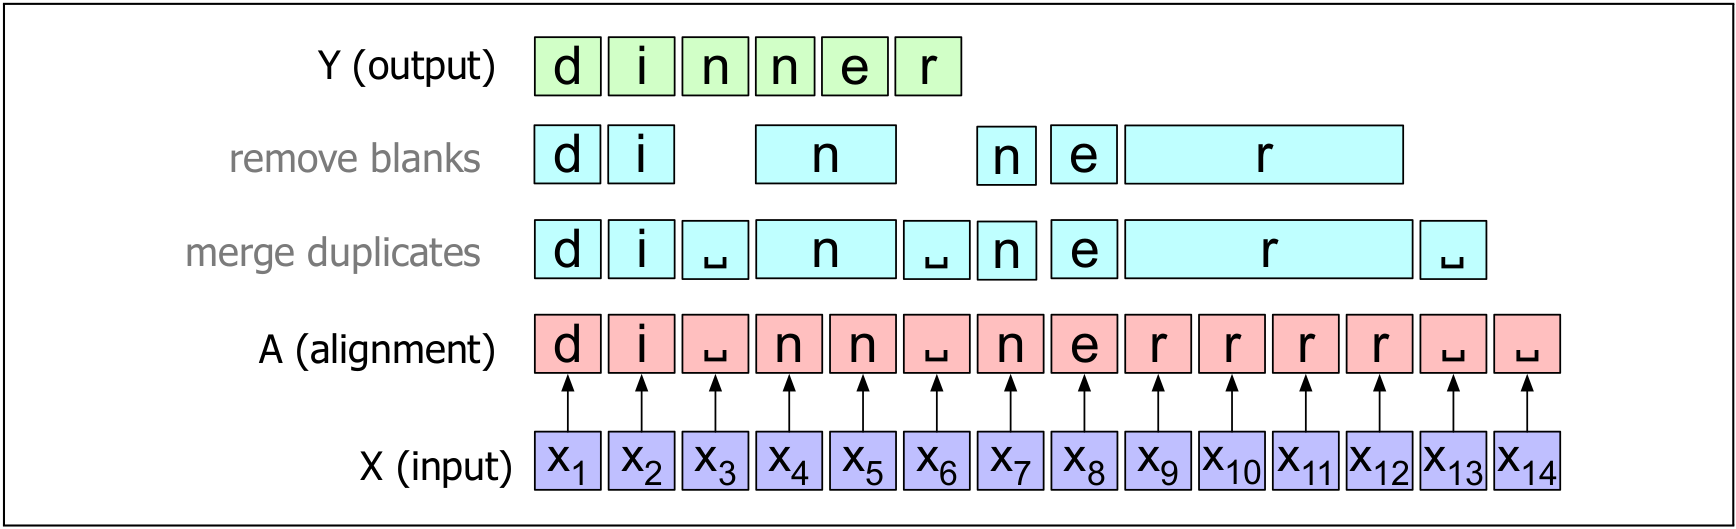
\includegraphics[width=0.8\textwidth]{ctc.png}
    \caption{A diagram that describes the alignment procedure of CTC \cite{jurafskyspeech}. \hl{TODO}: create own version of the same visual explanation and use the running example of ``The quick brown fox ...''.}
    \label{ctc}
\end{figure}

Given a sequence of speech features, CTC maps each speech feature to a single character, which results in a sequence of characters called an \emph{alignment}. 
Then, a \emph{collapsing function} is used to merge consecutive duplicate characters in the alignment.
The authors of CTC propose the use of a special characters called a \emph{blank}, which is represented by \textvisiblespace.
The blank character accounts for words that contain consecutive duplicate characters (such as ``dinner'' which contains two consecutive ``n'' characters).
With the addition of the blank character, the collapsing function is responsible for merging consecutive duplicate characters and removing all instances of blank characters.
Following the notation of \cite{jurafskyspeech}, we define the collapsing function as a mapping $B: A \rightarrow Y$ for an alignment $A$ and output string $Y$.
Notice that $B$ is many-to-one, since many different alignments can map to the same output string (see Figure~\ref{dinner}).

\begin{figure}[h!]
    \centering
    \captionsetup{justification=centering}
    
\includegraphics[width=0.8\textwidth]{dinner.png}
    \caption{Three different alignments that produce the same output string when using the CTC collapsing function \cite{jurafskyspeech}.}
    \label{dinner}
\end{figure}

In \cite{jurafskyspeech}, the set of all alignments that map to the same output string $Y$ is denoted as $B^{-1}(Y)$, 
where $B^{-1}$ is the inverse of the collapsing function.
This notation is useful for our explanation of CTC inference and training.

\subsection{CTC Inference}
Here we discuss how CTC models the probability of the output string $Y$ 
for a sequence of speech features $X = \{x^{(1)}, \dots, x^{(T)}\}$, 
denoted by $P_{\text{CTC}}(Y|X)$.
The conditional probability above can be expressed as the summation over the probabilities
of all possible alignments that produce the output string $Y$. 
Hence, we obtain the expression: 
\begin{equation}
    P_{\text{CTC}}(Y|X) = \sum\limits_{A \in B^{-1}(Y)} P(A|X).
\end{equation}

We still need an expression for $P(A|X)$.
To compute $P(A|X)$, CTC makes a strong conditional independence assumption. 
It assumes that each alignment character $a^{(t)} \in \{a^{(1)}, \dots, a^{(T)}\}$ 
is computed independently of all the other alignment characters.
Hence, we obtain the expression:
\begin{equation}
    P(A|X) = \prod\limits_{t=1}^{T} p(a^{(t)} | x^{(t)}).
\end{equation}

Now we can find the best possible alignment for a given $X$, by simply greedily choosing the most probable character at each time step.
We compute each alignment character $\{\hat{a^{(1)}}, \dots, \hat{a^{(T)}}\}$, apply the collapsing function, and obtain the output string $Y$.
However, there is an issue with the greedy approach described above. 
The issue is that the most probable output string $\hat{Y}$ may not correspond
with the most probable alignment sequence $\{\hat{a^{(1)}}, \dots, \hat{a^{(T)}}\}$.
The reason for this is that there are many possible alignments that lead to the same
output string. Therefore, the most probable output string $\hat{Y}$ for a given $X$ corresponds to the highest summation over the probabilities of all its
possible alignments:

\begin{align}
    \hat{Y} = \text{argmax}_Y P_{\text{CTC}}(Y|X) &= \text{argmax}_Y \left(\sum\limits_{A \in B^{-1}(Y)} P(A|X)\right) \\
                                                               &= \text{argmax}_Y \left(\sum\limits_{A \in B^{-1}(Y)} \prod\limits_{t=1}^{T} p(a^{(t)} | x^{(t)})\right).
\end{align}

There are many possible alignments, and summing over all the possible alignments is expensive and infeasible.
We can use dynamic programming to approximate this sum by using a modified version of Viterbi beam search. 
The beam search returns a user-specified number of potential output strings, 
and a loss function is used to score each output string.
The string with the best score is chosen as the final prediction.

\subsection{CTC Training}
To train a CTC-based ASR (Automatic Speech Recognition) system, 
the negative log-likelihood loss is employed in conjunction with 
a specialized CTC loss function. Formally, the loss for a dataset 
$D$ is represented as the cumulative sum of the negative log-likelihoods 
of the correct output $Y$ for each corresponding input $X$:
\begin{align}
    L_{\text{CTC}} &= \sum_{(X,Y) \in D} -\log P_{\text{CTC}}(Y|X) \\
                    &= \sum_{(X,Y) \in D} -\log \left( \sum_{A \in B^{-1}(Y)} \prod_{t=1}^{T} p(a^{(t)} | x^{(t)}) \right).
\end{align}

Once again, we cannot compute a summation over all the possible alignments.
The summation is efficiently computed using a variant of the \emph{forward-backward algorithm}.
A detailed explanation of the forward-backward algorithm used for training CTC is given in \cite{hannun2017sequence}.


\subsection{Improving CTC with a language model.} Because of the strong conditional independence assumption mentioned earlier,
CTC does not implicitly learn a language model over the data.
Therefore, it is typical that the CTC algorithm predicts a sentence that has obvious spelling mistakes.
We can mitigate this issue by using a seperate language model (LM).
This is done by adding an additional term in the CTC loss function and using interpolation weights that are tuned on a validation set:

\begin{equation}
    \textit{score}_{\text{CTC}}(Y|X) = \log\left(P_{\text{CTC}}(Y|X)\right) + \lambda_1 \log\left(P_{\text{LM}}(Y)\right) + \lambda_2 L(Y).
\end{equation}

We have now discussed everything we need to know to create a self-supervised learning-based ASR model. 
First, we pre-train our model using wav2vec 2.0 and a large corpus of unlabeled data, 
and then we fine-tune our model using CTC.
However, in the following section will discuss a major issue with this approach.
We will also discuss how our approach differs from the approach above.



% ***************************************************
% SECTION 4
% ***************************************************
\section{Fine-tuning existing wav2vec 2.0 models}
Pre-training with wav2vec 2.0 using unlabeled data is infeasible for our study because:
\begin{enumerate}
    \item Pre-training with wav2vec 2.0 is known to be quite unstable (see ``NOTE 1'' of \cite{vonplaten2021pretraining}).
    \item Performing one experiment (run) of the large-scale wav2vec 2.0 model, using 8 GPU V100s (16 GB RAM each), takes 7 days to finish \cite{vonplaten2021pretraining}.
\end{enumerate}
At the time of conducting this study, we did not have access to the computational resources required to perform pre-training experiments.
This is why our study focuses on fine-tuning existing pre-trained wav2vec 2.0 models, rather than performing pre-training and then fine-tuning.
In this section, we discuss two pre-trained models used in this study: Wav2Vec2-Large and XLS-R.

\subsection{Wav2Vec2-Large}
\hl{TODO}: Need to make sure about the choice of model here. One option: \href{https://huggingface.co/facebook/wav2vec2-large}{Wav2Vec2-Large}.

\subsection{XLS-R}
XLS-R \cite{babu2021xls} is a large-scale wav2vec 2.0 model trained on 128 different languages to learn \emph{cross-lingual} speech representations.
XLS-R attempts to build better representations for low-resource languages by leveraging cross-lingual transfer from high-resource languages such as English.

The model is trained using batches that contain samples from multiple languages $L$. 
Batches are sampled from a probability distribution $p_l \sim \left(\dfrac{n_l}{N}\right)^{a}$ where:
\begin{itemize}
    \item $l \in \{1, \dots, L\}$ represents each language.
    \item $N$ is the number of hours of all the unlabeled data and $n_l$ is the number of hours of unlabeled data for the language $l$.
    \item $\alpha$ controls how much data is chosen from the high-resource and low-resource languages.
\end{itemize}

The total number of hours of all the unlabeled data combined is about 436K hours. The authors used data from 24 high-resource languages, 17 mid-resource languages, and 88 low-resource languages.
The high-resource languages contain more than 1K hours of data each, the mid-resource languages contain more than 100 hours (but less than 1K hours)
of data each, and the low-resource languages contain less than 100 hours of data each.

XLS-R is evaluated on a wide range of downstream tasks: ASR, automatic speech translation (AST), and speech classification which includes language identification and speaker identification.
The evaluation results at the time improved on the previous state of the art for several benchmarks for every downstream task. 
This demonstrates the generalization ability of XLS-R.